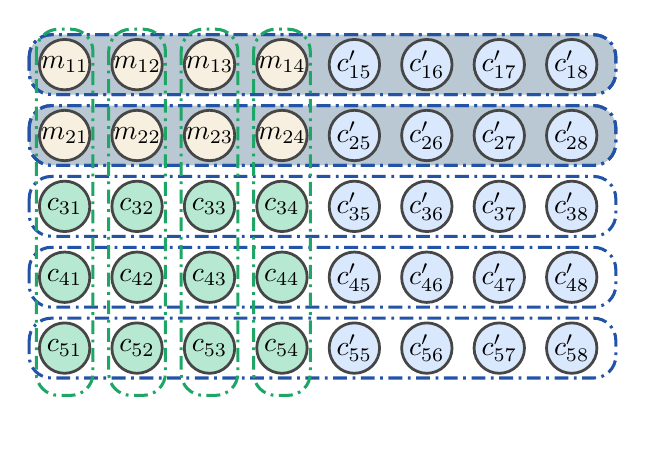
\begin{tikzpicture}[x=1cm,y=1cm]

% Colors (approximate to the figure)
\definecolor{dashblue}{RGB}{34,83,167}
\definecolor{dashgreen}{RGB}{30,166,103}
\definecolor{cream}{RGB}{247,239,224}
\definecolor{mint}{RGB}{183,232,210}
\definecolor{sky}{RGB}{212,233,246}
\definecolor{stroke}{RGB}{70,70,70}

% --- Colors (same style as yours) ---
\definecolor{bgblue}{RGB}{235, 245, 255}
\definecolor{nodeblue}{RGB}{212,233,246}
\definecolor{nodecream}{RGB}{247,236,214}
\definecolor{nodegreen}{RGB}{221,244,234}
\definecolor{borderblue}{RGB}{100, 149, 237}
\definecolor{bordergreen}{RGB}{46, 125, 50}
\definecolor{textblue}{RGB}{0, 51, 102}
\definecolor{arrowgray}{RGB}{128, 128, 128}
\definecolor{edgegray}{RGB}{140,140,140}

\definecolor{rainbowyellow}{HTML}{FFF3CE}
\definecolor{rainbowgreen}{HTML}{D6E9D5}
\definecolor{rainbowred}{HTML}{FAD8D4}
\definecolor{rainbowcyan}{HTML}{AFE3E6}
\definecolor{rainbowblue}{HTML}{D9E8FC}
\definecolor{rainbowgray}{HTML}{BAC8D3}

% Parameters
\pgfmathsetmacro\rows{5.0}
\pgfmathsetmacro\cols{8.0}
\def\dx{0.92}
\def\dy{0.90}
\def\r{0.32}
\def\left{0}
\def\top{0}
\pgfmathsetmacro{\ybottom}{-(\rows-1)*\dy - 0.60}

% Helper: circle fill by row/col
% Row index i = 1..7 from top to bottom; col j = 1..7 from left to right.
\foreach \i in {1,...,5} {
  % y coordinate for row
  \pgfmathsetmacro{\yy}{-(\i-1)*\dy}

   
  % Long dashed blue rounded rectangle for each row
   \pgfmathtruncatemacro{\drawenc}{(\i==1) || (\i==2)}
   \ifnum \drawenc=1
     \draw[draw=dashblue, line width=1.1pt, dash pattern=on 5pt off 2pt on 1pt off 2pt, fill=rainbowgray,
        rounded corners=8pt]
    (-0.45, \yy+0.38) rectangle (7.0, \yy-0.38);
    \fi


  % Circles
  \foreach \j in {1,...,4} {
        \pgfmathsetmacro{\xx}{(\j-1)*\dx}
    
        % Decide fill color
        % First 3 columns: top 3 rows cream, bottom 4 rows mint.
        % Last 4 columns: all sky.
          \ifnum\i<3
            \def\fillcol{cream}
          \else
            \def\fillcol{mint}
          \fi

          
        \draw[draw=stroke, line width=1pt, fill=\fillcol] (\xx, \yy) circle (\r);

        \ifnum\i<3
            \node[anchor=center, font=\selectfont] at (\xx, \yy) {$m_{\i\j}$};
        \else
            \node[anchor=center, font=\selectfont] at (\xx, \yy) {$c_{\i\j}$};
        \fi
            
    }

    % Draw Code2
    % \ifnum \drawenc=1
        \foreach \j in {5,...,8} {
            \pgfmathsetmacro{\xx}{(\j-1)*\dx}
            \def\fillcol{rainbowblue}
            \draw[draw=stroke, line width=1pt, fill=\fillcol] (\xx, \yy) circle (\r);
              \node[anchor=center, font=\selectfont] at (\xx, \yy) {$c_{\i\j}'$};
          }
          \draw[draw=dashblue, line width=1.1pt, dash pattern=on 5pt off 2pt on 1pt off 2pt, rounded corners=8pt]
        (-0.45, \yy+0.38) rectangle (7.0, \yy-0.38);
    % \fi
}


% Three vertical dashed green rounded rectangles over the first 3 columns
\foreach \j in {1,...,4} {
  \pgfmathsetmacro{\xleft}{(\j-1)*\dx - 0.36}
  \pgfmathsetmacro{\xright}{(\j-1)*\dx + 0.36}

  \draw[
    draw=dashgreen,
    line width=1.1pt,
    dash pattern=on 5pt off 2pt on 1pt off 2pt,
    rounded corners=8pt
  ]
    (\xleft,0.45) rectangle (\xright,\ybottom);
}



% Bottom text: Enc^{\otimes \epsilon^{-1}} \ldots Enc^{\otimes \epsilon^{-1}}
\node[anchor=center, font=\large\selectfont] at (1.5, -4.55) {$\Enc~~\Enc~~\Enc~~\Enc$};
\end{tikzpicture}